\documentclass{article}

\usepackage{kotex}
\usepackage{graphicx}
\usepackage[affil-it]{authblk}
\usepackage{mathtools}
\usepackage{amssymb}
\usepackage{amsthm}
\usepackage{geometry}
\usepackage{fancyhdr}
\usepackage{braket}
\usepackage{cite}
\usepackage{cancel}
\usepackage{subcaption}
\usepackage{enumitem}
\usepackage{color}
\usepackage{chemformula}
\usepackage{physics}
\usepackage{hyperref}

\newcommand{\vp}{\varphi}
\newcommand{\ve}{\varepsilon}

\theoremstyle{definition}
\newtheorem{theorem}{Theorem}
\newtheorem{definition}[theorem]{Definition}
\newtheorem{example}[theorem]{Example}
\newtheorem{lemma}[theorem]{Lemma}
\newtheorem{axiom}[theorem]{Axiom}
\newtheorem{remark}[theorem]{Remark}
\newtheorem{problem}[theorem]{Problem}
\newtheorem{exercise}[theorem]{Exercise}

\counterwithin{equation}{section}
\counterwithin{theorem}{section}


\geometry{a4paper,left=2cm,right=2cm,top=2.4cm,bottom=2.4cm}

\linespread{1.3}

\title{\textsf{Introduction to Statistic}}
\author[1]{Written by Eun Taek Kang\thanks{email: etkang03@gmail.com}}
\affil[1]{Department of Physics, Sogang University, Seoul 04107, Korea}

\date{Summer 2025, Sogang University}

\begin{document}

\pagestyle{fancy}
    %... then configure it.
    \fancyhf{}
    % Set the header and footer for Even
    % pages but omit the zone (L, C or R)
    \fancyhead[R]{\textsf{Prof.\ Kyungpil Lim}}
    \fancyhead[L]{\textsc{Introduction to Statistic}}
    \fancyfoot[C]{\thepage}
    \fancyfoot[L]{\textbf{Sogang University}}
    \fancyfoot[R]{\textit{Department of Mathematics}}

\maketitle

\begin{abstract}
    본 문서는 서강대학교의 2025년 하계학기 통계학입문 강의의 내용을 필기하고 정리한 노트입니다. 모든 내용은 임경필 교수님의 강의를 바탕으로 작성되었습니다.
\end{abstract}

\newpage

\section{확률}

\subsection{확률의 정의}

\textbf{확률현상, 확률실험}

\begin{itemize}
    \item 확률현상(random phenomenon) : 불확실성에 의해서 좌우되는 현상
    \item 확률실험(random experiment) : 결과가 불확실성에 의해 좌우되는 실험이나 조사
\end{itemize}

\begin{example}[확률현상의 예]
    확률 현상의 예시들은 다음과 같다.

    \begin{enumerate}
        \item 동전이나 주사위를 던질 때 결과가 나타나는 현상
        \item 각 지역에서의 연 강수량의 변동 현상
        \item 수시로 달라지는 주가의 변동 현상
        \item 월 생산품에 포함되는 불량품(수)의 출현 현상
    \end{enumerate}
\end{example}

\noindent
\textbf{표본공간, 표본점, 사건}

\begin{enumerate}
    \item \textcolor{red}{표본공간}(sample space; $\Omega$) : 한 확률실험에서 얻어질 수 있는 가능한 모든 결과의 집합. 표본공간 = 전공간
    \item \textcolor{red}{표본점}(sample point; $\omega_i$) : 표본공간의 원소 하나
    \item \textcolor{red}{사건}(event) = \textcolor{red}{사상} : 표본공간의 부분집합
    \item \textcolor{red}{근원사건}(elementary event)= \textcolor{red}{단순사건}(simple event) : 표본점 하나하나로 이루어지는 사건
\end{enumerate}

\begin{example}
    확률실험에 대한 표본공간의 예시는 다음과 같다.

    \begin{enumerate}
        \item 하나의 동전을 던지고 윗면에 나타나는 상태를 관찰하는 확률실험: (단, Heads(앞면-그림), Tails(뒷면-금액))
        
        표본공간 : $\Omega = \{ H, T \}$

        \item 하나의 주사위를 던지고 윗면에 나타나는 점의 개수를 관찰하는 확률실험:
        
        표본공간 : $\Omega = \{1,2,3,4,5,6 \}$
    \end{enumerate}
\end{example}

\noindent
우리는 셀 수 있는 공간(countable)뿐 아니라 셀 수 없는 공간(uncountable)에서의 확률도 고려해야 한다. 이때 등장하는 것이 \textbf{기하적 확률}(Ex. 길이, 넓이, 부피)이다.\footnote{이런 부분은 실해석학(Real Analysis)의 공부에 도움이 된다.}

\vspace{4mm}\noindent
주사위를 굴려서 짝수가 나온다는 확률을 잴 때, \{2\}, \{4\}, \{6\}으로 쪼개지 \{2, 4\}, \{4, 6\}으로 굳이 쪼개어 생각하지 않는다. 따라서 이후 나올 배반사건으로 쪼개서 생각하는 것이 상당히 중요한 사고로 작용한다.

\newpage

\noindent
\textbf{사건의 결합(combination of events)}

\begin{enumerate}
    \item 여사건: $E_1^c$
    \item 합사건: $E_1 \cup E_2$
    \item 교사건: $E_1 \cap E_2 = E_1 E_2$\footnote{중간의 교집합 기호를 생략할 수 있다. Cartesian product가 아님에 유의하자.}
    \item 차사건: $E_1 - E_2$
    \item 무한가산합사건: $\bigcup_{i=1}^\infty E_i = \{ \omega \in \Omega \ | \ \exists \ i \in \mathbb{N}, \ \omega \in E_i \}$
    \item 무한가산교사건: $\bigcap_{i=1}^{\infty} E_i = \left\{ \omega \in \Omega \;\middle|\; \forall \ i \in \mathbb{N},\; \omega \in E_i \right\} $
\end{enumerate}

\noindent
\textbf{사전확률, 사후확률}

\begin{itemize}
    \item \textcolor{red}{사전확률} : 확률실험에서 모든 결과가 같은 가능성을 갖고 일어난다고 하자. 이 실험에서 일어날 수 있는 가능한 모든 결과의 수가 $N$, 또 한 사건 $E$를 일어나게 하는 결과의 수가 $n$이면, 이때 사건 $E$가 일어날 확률은 $P(E) = n/N$이다. 
    \item \textcolor{red}{사후확률} : 한 확률실험을 반복한 총 횟수를 $N$ 이라 하고, 또 그 중 사건 $E$를 일어나게 한 실험의 횟수를 $n$이라 하면, 이때 사건 $E$가 일어날 확률은 $P(E) = \lim_{N \rightarrow \infty} n/N$이다.
\end{itemize}

\noindent
\textbf{배반사건(mutually exclusive events)}

\begin{definition}
    두 사건 $E_1$과 $E_2$가 $E_1 \cap E_2 = \emptyset$을 만족할 때, $E_1$과 $E_2$는 상호 \textcolor{red}{배반사건}이라 한다.
\end{definition}

\noindent
경우의 수와 확률을 분석할 때, 상호 배반사건 관계에 있는 것들로 쪼개주는 것이 중요하다. 윷놀이 예시가 있는데 한 번쯤 분석해보도록 합시다.

\vspace{5mm}\noindent
\textbf{공리론적 확률}

\noindent
정의역때문에 설명이 어려워서 그냥 대충 받아들이고 가도 무방하나, 실해석학할 때 도움된다. (실사몇하;;)

\begin{definition}
    $\Omega$를 확률실험의 표본공간이라 하고, $\mathcal{F}$를 $\Omega$ 위에서 정의된 사건들의 `$\sigma$-집합체'라고 할 때, 집합함수 $P : \mathcal{F} \rightarrow \mathbb{R}$ ($\mathcal{F} \subset P(\Omega)$)가 다음 세 가지 조건을 만족할 때 $P$를 \textcolor{red}{확률함수}(probability function)라 하고, ($\Omega, \mathcal{F}, P$)를 \textcolor{red}{확률공간} (probability space)이라 한다.

    \begin{enumerate}
        \item[(A1)] $\forall E \in \mathcal{F}$, $P(E) \geq 0$
        \item[(A2)] 임의의 배반사건인 $\{E_n\}_{n=1}^\infty \subset \mathcal{F}$에 대하여,
        \begin{equation*}
            P \left( \bigcup_{n=1}^\infty E_n \right) = \sum_{n=1}^\infty P(E_n)
        \end{equation*} 
        \item[(A3)] $P(\Omega)=1$
    \end{enumerate}
\end{definition}

\noindent
상호 배반 합집합의 경우, (A2)의 $\cup$의 중간에 점을 찍어 표현하기도 한다. 이러한 공리론적 확률덕분에 배반사건에 대해서 합을 구하는 것은 상당히 쉽게 된다.

\newpage

\noindent
\textbf{$\sigma$-집합체($\sigma$-field), $\sigma$-집합대수($\sigma$-algebra)}

\begin{definition}
    $\Omega$를 확률실험의 표본공간이라 하고, $\mathcal{F}$를 $\Omega$의 부분 집합족이라 할 때, 다음 세가지 조건을 만족할 때 $\mathcal{F}$를 $\Omega$ 위에서의 \textcolor{red}{$\sigma$-집합체} 또는 \textcolor{red}{$\sigma$-집합대수}라 한다.

    \begin{enumerate}
        \item[(i)] $E \in \mathcal{F} \Rightarrow E^c \in \mathcal{F}$
        \item[(ii)] 임의의 $\mathcal{F}$의 가산무한 사건열 $\{E_n\}_{n=1}^\infty$에 대하여
        \begin{equation*}
            \bigcup_{n=1}^\infty E_n \in \mathcal{F}
        \end{equation*}

        \item[(iii)] $\emptyset \in \mathcal{F}$
    \end{enumerate}
\end{definition}

\begin{theorem}[$\sigma$-집합체의 기본 성질]
    $\mathcal{F}$를 $\Omega$ 위에서의 $\sigma$-집합체라 하자.

    \begin{enumerate}
        \item $\Omega \in \mathcal{F}$
        \item 임의의 $\mathcal{F}$의 가산무한 사건열 $\{E_n\}_{n=1}^\infty$에 대하여
        \begin{equation*}
            \bigcap_{n=1}^\infty E_n \in \mathcal{F}
        \end{equation*}
    \end{enumerate}
\end{theorem}

\begin{definition}[Borel $\sigma$-집합체]
    \(\mathbb{R}\)의 부분집합들의 집합족 \(\{(-\infty, x] \mid x \in \mathbb{R} \}\)를 포함하는 \(\mathbb{R}\) 위에서의 가장 작은 \(\sigma\)-집합체 \(\mathcal{B}\)를 \textcolor{red}{Borel \(\sigma\)-집합체}라고 한다. 
    Borel \(\sigma\)-집합체 \(\mathcal{B}\)는 \(\mathbb{R}\)의 모든 형태의 구간, 즉, 다음과 같은 형태의 구간을 포함한다.
    \begin{equation*}
        (-\infty, a], \quad (-\infty, a), \quad [a, \infty), \quad (a, \infty), \quad (a, b), \quad  (a, b], \quad [a, b), \quad [a, b]
    \end{equation*}
    여기서,
    \begin{equation*}
        (-\infty, a) = \bigcup_{n \in \mathbb{N}} \left(-\infty, a - \dfrac{1}{n} \right]
    \end{equation*}
\end{definition}

\begin{theorem}
    $(\Omega, \mathcal{F}, P)$가 확률공간일 때,

\begin{enumerate}
  \item 임의의 상호 배반인 $\mathcal{F}$의 유한 사건열 $\{E_1, E_2, \dots, E_n\}$에 대하여
  \[
  P(E_1 \cup E_2 \cup \cdots \cup E_n) = P\left( \bigcup_{i=1}^n E_i \right) = \sum_{i=1}^n P(E_i)
  \]

  \item $\forall E \in \mathcal{F}, \quad P(E^c) = 1 - P(E)$

  \item $\forall E \in \mathcal{F}, \quad 0 \leq P(E) \leq 1$

  \item $P(\emptyset) = 0$
\end{enumerate}
\end{theorem}

\begin{proof}
    ($\Omega, \mathcal{P}, P$) : 확률 공간

    \noindent
    (1) : 증명은 생략한다.

    \noindent
    (2) : $E \cup E^c = \Omega$이고, $E \cap E^c = \emptyset$ (상호 배반)이므로, (A2)에 의해 $P(E\cup E^c) = P(E) + P(E^c)$이고, (A3)에 의해 $P(\Omega) = 1$이다. $P(E \cup E^c) = P(\Omega)$이므로, $P(E^c) = 1-P(E)$이 증명된다.

    \noindent
    (3) : (A1)에 의하여 $P \geq 0$이 성립한다. (2)에서 얻었던 점에 의하여 $P(E) = P(\Omega) - P(E^c)$였다. 따라서, 부등식을 세울 수 있다. $P(E) \leq P(\Omega) = 1$ 따라서, 두 부등식을 종합하면 $0 \leq P(E) \leq 1$이 증명된다.

    \noindent
    (4) : $\Omega = \Omega \cup \emptyset$이다. 둘은 상호 배반이므로 $P(\Omega) = P(\Omega) + P(\emptyset)$이다. 따라서 $P(\emptyset) = 0$이 증명되었다. 
\end{proof}

\noindent
우리는 항상 확률을 $\sigma$-집합체 위에서 정의할 것이다. 확률을 취할 수 있는 사건들만 생각하자.

\noindent
\textcolor{blue}{\textbf{[6/24, Lecture 1 to here]}}

\newpage

\noindent
앞서 배운 상호 배반 관계의 합집합에선 계산이 공리에 의해 매우 간단했다. 그러나, 일반적인 합집합에 대한 확률은 어떻게 될까? 이는 합의 법칙을 통해 설명할 수 있다.

\begin{theorem}[합의 법칙]
    ($\Omega, \mathcal{F}, P$)가 확률공간이면 임의의 $E_1, \cdots, E_n \in \mathcal{F}$에 대하여,
    \begin{equation*}
        P\left( \bigcup_{i=1}^{n} E_i \right) = \sum_{i=1}^{n} P(E_i) - \sum_{i<j} P(E_i \cap E_j) + \sum_{i<j<k} P(E_i \cap E_j \cap E_k) + \cdots + (-1)^{n+1} P(E_1 \cap E_2 \cap \cdots \cap E_n)
    \end{equation*}

    \begin{itemize}
        \item $P(E_1 \cup E_2) = P(E_1) + P(E_2) - P(E_1 \cap E_2)$
        \item $P(E_1 \cup E_2 \cup E_3) = P(E_1) + P(E_2) + P(E_3) - P(E_1 \cap E_2) - P(E_1 \cap E_3) - P(E_2 \cap E_3) + P(E_1 \cap E_2 \cap E_3)$
    \end{itemize}
\end{theorem}

\begin{proof}
    $n=2$인 경우에 대해 해보자. Claim : $P(E_1 \cup E_2) = P(E_1) + P(E_2) - P(E_1 \cap E_2)$

    \noindent
    공리를 사용하기 위하여 우리는 상호 배반인 관계로 분리하는 것이 유리하다. 두 집합을 $E_1, E_2 \cap E_1^c$로 나누자.
    \begin{equation*}
        E_1 \cup E_2 = E_1 \dot{\cup} (E_2 \cap E_1^c) \quad / \quad E_2 = (E_1 \cap E_2) \dot{\cup} (E_2 \cap E_1^c)
    \end{equation*}
    따라서, 확률로써 정리하고 양 변을 빼주면 다음과 같다.
    \begin{equation*}
        \begin{cases}
            P(E_1 \cup E_2) = P(E_1) + P(E_2 \cap E_1^c)\\ P(E_2) = P(E_1 \cap E_2) + P(E_2 \cap E_1^c)
        \end{cases} \quad \Rightarrow \quad P(E_1 \cup E_2) = P(E_1) + P(E_2) - P(E_1 \cap E_2)
    \end{equation*}
    따라서 $n=2$일 때의 합의 법칙이 증명되었다.
\end{proof}

\noindent
확률의 합은 같은 counting measure이기 때문에, 유한집합의 개수와 연산의 양상이 상당히 비슷하다.

\begin{example}
    한 개의 좋은 주사위를 두 번 던지는 확률실험에서, 첫 번째 결과에서 점의 개수가 2를 넘지 않거나 두 번째 결과에서 점의 개수가 적어도 5가 될 확률을 구하시오.
\end{example}

\noindent
\textbf{Solution:} $\Omega = \{ (a, b) | a, b = 1, 2, \cdots 6 \}$ / $\mathcal{F} = \mathcal{P} (\Omega) = \Omega$의 모든 부분집합의 모임 / $P(\{ (a,b) \} ) = \frac{1}{36}$, $\forall (a, b) \in \Omega$ 이때, 사건 $E_1, E_2$를 다음과 같이 정의할 수 있다.
\begin{align*}
    E_1 &= \text{첫 번째 결과에서 점의 개수가 2를 넘지 않을 사건}\\
    E_2 &= \text{두 번째 결과에서 점의 개수가 적어도 5가 될 사건}
\end{align*}

\begin{definition}[조건부 확률(conditional probability)]
    확률공간 ($\Omega, \mathcal{P}, P$)에서, $E_1, E_2 \in \mathcal{F}$이고, $P(E_2) > 0$일 때 사건 $E_2$가 일어났다는 조건에서 사건 $E_1$이 일어날 확률을 \textcolor{red}{사건 $E_2$에 대한 사건 $E_1$의 조건부 확률}이라 하며, $P(E_1 | E_2)$로 나타내고 다음과 같이 정의한다.
    \begin{equation*}
        P(E_1 | E_2)_ = \frac{P(E_1 \cap E_2)}{P(E_2)} = \frac{P(E_1 E_2)}{P(E_2)}
    \end{equation*}
\end{definition}

\noindent
다음 그림을 한 번 떠올려보자.
\begin{figure}[h]
    \centering
    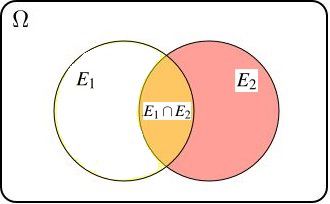
\includegraphics[width = 0.3\linewidth]{image/fig1_1.png}
\end{figure}

\noindent
교집합을 의미하는 것 자체는 똑같으나, \underline{전체 사건(분모)를 어떻게 잡아주냐}의 차이이다! 조건부 확률에 정의에서 확률의 곱의 법칙이 나온다. 조건부확률은 Local한 개념이고, $P(E_1 | E_2)$와 $P(E_2 | E_1)$은 서로 다르다.

\noindent
$\Omega$ 위에서 확률을 정리했는데, $E_2$로 범위를 줄여서 논해도 확률함수인가? 이를 보증해주는 것이 조건부 확률 정의의 타당성이다. 이는 vector space와 subspace 간의 관계와 구조가 일치한다. 확률함수가 만족하는 성질들을 subspace에 대해서도 모두 만족시켜줄 수 있다.

\newpage

\begin{theorem}[조건부 확률 정의의 타당성]
    $(\Omega, \mathcal{F}, P)$가 확률 공간이면, $P(B) > 0$인 임의의 사건 $B \in \mathcal{F}$에 대하여, 집합함수 $P(\ \cdot \mid B) : \mathcal{F} \to \mathbb{R}$는 확률함수이다. 즉, $(\Omega, \mathcal{F}, P|_{B})$는 확률 공간이다.
\end{theorem}

\begin{proof}
    (A1) : $\forall E \in \mathcal{F}$, $P(E|B) = P(E \cap B) / P(B) \geq 0 $
    \\ \noindent (A2) : 임의의 상호 배반인 $\{E_n\}_{n=1}^\infty \subset \mathcal{F}$에 대하여 (여기 뒤에는 필기 보고 채워넣어라)
    \\ \noindent (A3) : 
    \begin{equation*}
        P(\Omega | B)  = \frac{P(\Omega \cap B)}{P(B)} = \frac{P(B)}{P(B)} = 1
    \end{equation*}
\end{proof}

\begin{theorem}[곱의 법칙]
    $(\Omega, \mathcal{F}, P)$가 확률공간이고, $E_1, E_2, \cdots, E_n \in \mathcal{F}$, $P(E_1 \cap E_2 \cap \cdots \cap E_n) > 0$이면,\footnote{조건부 확률의 곱이기 때문에 양수 조건 빼먹으면 안된다!!, 얘가 양수면 나머지 확률들도 양수임이 보장된다.}
    \begin{equation*}
        P(E_1 \cap E_2 \cap \cdots \cap E_n) = P(E_1) P(E_2 \mid E_1) \cdots P(E_n \mid E_1 \cap E_2 \cap \cdots \cap E_{n-1})
    \end{equation*}
    특히, $n=3$이면,
    \begin{equation*}
        P(E_1 \cap E_2 \cap E_3) = P(E_1) P(E_2 \mid E_1) P(E_3 \mid E_1 \cap E_2)
    \end{equation*}
\end{theorem} 

\begin{proof}
    Use Mathematical Induction.\\
    \noindent
    (i) $n=2$, $P(E_1 \cap E_2) = P(E_1) \cdot P(E_2 | E_1)$ (정의)\\
    \noindent
    (ii) $n=k$일 때, 성립한다고 가정하면,
    \begin{align*}
        P(E_1 \cap E_2 \cap \cdots \cap E_n \cap E_{n+1}) &=  P(E_1 \cap \cdots \cap E_k) \cdot P(E_{k+1} \mid E_1 \cap \cdots \cap E_k)\\
        &= P(E_1) P(E_2 \mid E_1) \cdots P(E_k \mid E_1 \cap \cdots \cap E_{k-1}) \cdot P(E_{k+1} \mid E_1 \cap \cdots \cap E_k)
    \end{align*}
    따라서, 수학적 귀납법에 따라, 임의의 자연수 $n$에 대해 곱의 법칙이 성립한다.
\end{proof}

\begin{example}
    주머니 안에 3개의 검은 공과 7개의 흰 공이 있는데, 1개씩 2번 뽑아서 두 개 모두 검은 공이 나올 확률은 얼마인가? (Naive하게 $\frac{3}{10} \times \frac{2}{9}$가 될 것이다.)
\end{example}

\noindent
\textbf{Solution:} $B_i$는 $i$번째에 검은 공을 뽑는 사건이다. 구하는 것은 $P(B_1 \cap B_2)$이 된다.
\begin{equation*}
    P(B_1 \cap B_2) = P(B_1) \cdot P(B_2 | B_1)
\end{equation*}
양 변에 $P(B_1)$을 나눠보면 명확히 조건부 확률의 정의가 된다.


\begin{example}
    상자 안에 30개의 전구가 있는데 그 중 5개는 불량품이다. 3개를 비복원추출한다고 할 때, 3개 모두 불량품일 확률을 구하시오. (Naive하게 $\frac{5}{30} \times \frac{4}{29} \times \frac{3}{28}$이 될 것이다.)
\end{example}

\noindent
\textbf{Solution:} $B_i$는 $i$번째에 불량품을 뽑는 사건이다. 구하는 것은 $P(B_1 \cap B_2 \cap B_3)$이 된다.
\begin{equation*}
    P(B_1 \cap B_2 \cap B_3) = P(B_1) \cdot P(B_2 | B_1) \cdot P(B_3 | B_1 \cap B_2)
\end{equation*}

\newpage

\begin{definition}[표본공간의 분할(partition)]
    확률공간 $(\Omega, \mathcal{F}, P)$에서 $\mathcal{F}$의 유한 또는 무한가산 사건열 $\{E_i\}_{i \in I}$가 다음 조건을 만족할 때, $\{E_i\}_{i \in I}$를 \textcolor{red}{표본공간 $\Omega$의 분할}이라고 한다.
    \begin{enumerate}
        \item[(i)] 임의의 $i, j \in I$에 대하여 $i \ne j$이면 $E_i \cap E_j = \emptyset$이다.
        \item[(ii)] \(\displaystyle \bigcup_{i \in I} E_i = \Omega\)
    \end{enumerate}
\end{definition}

\begin{figure}[h]
    \centering
    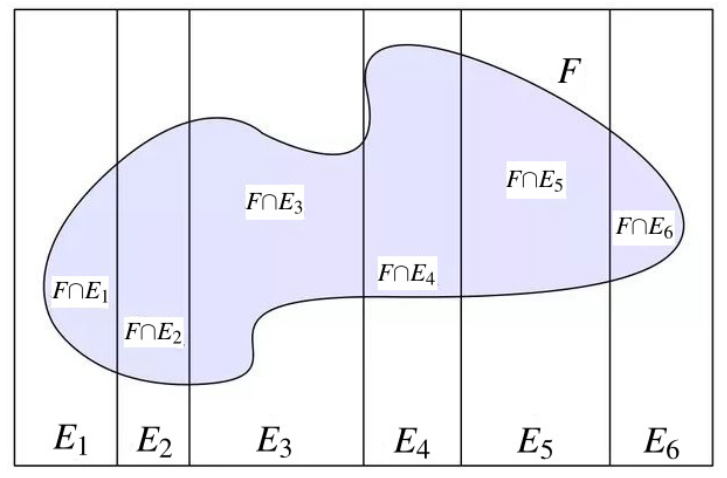
\includegraphics[width = 0.4\linewidth]{image/fig1_2.png}
\end{figure}

\noindent
표본공간의 분할에 관한 자세한 예는 필기를 보고 채워 넣자.

\begin{theorem}
    확률공간 $(\Omega, \mathcal{F}, P)$에서 $\{E_i\}_{i \in I}$는 표본공간 $\Omega$의 분할이고, $\forall i \in I$, $P(E_i) > 0$ 라고 하자.
    \begin{itemize}
        \item \textcolor{red}{전확률의 법칙}(rule of total probability) :
        \[
        \forall F \in \mathcal{F}, \quad P(F) = \sum_{i \in I} P(E_i) P(F \mid E_i)
        \]
        \item \textcolor{red}{베이즈의 법칙}(Bayes' rule) : $F \in \mathcal{F}$이고 $P(F) > 0$이면,
        \[
        P(E_j \mid F) = \frac{P(E_j) P(F|E_j)}{P(F)}= \frac{P(E_j) P(F \mid E_j)}{\sum_{i \in I} P(E_i) P(F \mid E_i)}
        \]
    \end{itemize}
\end{theorem}

\begin{example}
    두 개의 항아리가 있다. 첫째 항아리에는 노란 구슬 2개와 빨간 구슬 4개가 들어있고 둘째 항아리에는 노란 구슬 3개와 빨간 구슬 5개가 들어있다. 둘째 항아리에서 하나의 구슬을 꺼내어 첫째 항아리에 넣고 첫째 항아리에서 하나의 구슬을 꺼낼 때 노란 구슬이 나올 확률을 구하시오.
\end{example}

\noindent
\textbf{Solution:}

\noindent
\textcolor{blue}{\textbf{[6/25, Lecture 2 to here]}}

\end{document}